%
% $Id: conclusion.tex
%
%   *******************************************************************
%   * SEE THE MAIN FILE "AllegThesis.tex" FOR MORE INFORMATION.       *
%   *******************************************************************
%

\chapter{Discussion and Future Work}\label{ch:conclusion}
This chapter outlines how the current state of the project compares to the original
proposal, including shortcomings and changes in the vision. It finishes with a reflection
on the application.

\section{Future Work}
The vision I have for the final version of this application is far beyond what
I was able to accomplish in one semester. I would like to eventually create a
fully functional web app, with a variety of options in the hopes of using as
much of the Spotify API as possible.

Due to the time constraints associated with this thesis project, the current
release is lacking many features that I expect the final application to include.
The biggest compromise was in the web page user interface, as I did not have the
time to configure every file to work with the Flask framework. Despite this, I am
encouraged that my first attempt works correctly, which should serve to make
future work easier, or at the least more familiar. If this project is to be used
by the general public, it is a necessity to be hosted on a website, with a user
interface that is both easy to understand and use. For this reason, creating an
entirely web-based application is the most pressing change to work on in the future.

Due to the structure of this project, it is conducive to add new features, without
having to weaken the integrity of the overall project. As such, the next feature
I would like to add is to trawl playlists for songs, by requesting a keyword from
the user. This would allow users to just type in a word, and receive songs that
other users have put in playlists related to the term. Since playlists are a
major part of Spotify, and contain songs chosen by users, instead of algorithms
alone, this is a powerful resource, which arrives pre-sorted. Therefore, choosing
songs from playlists will likely add a level of accuracy, and likeliness of
enjoyment, that is difficult to replicate by automation alone.

Another feature which I consider very important, especially for public use, is
mobile support. Again due to time, I did not have the opportunity to look into how
to develop for mobile, but I did learn that Flask can be used for mobile app
back-end. This is also encouraging for the final stage of this project. Like
much of the current internet, Spotify relies heavily on mobile usage. This is an
area I would like Scottipy to be able to access and address, but will require more
work.

A more conceptual change to investigate is to investigate Spotify user behavior,
in order to match this project with how users treat Spotify. In a paper focused
on this user behavior, user trends, and differences between desktop and mobile
usage were found \cite{6566767}. For one, the research team found that desktop
and mobile sessions peaked at different times through the day, and also in
different amounts; where destop sessions tended to peak higher than mobile, in
terms of percentage of total Spotify users.

\begin{center}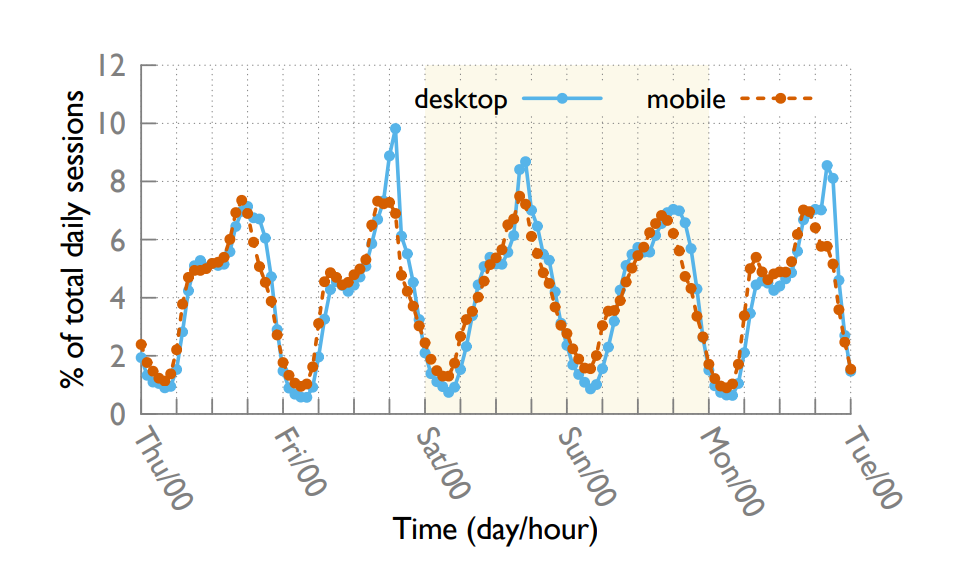
\includegraphics[height=9cm]{images/trends.png}
\end{center}

These tendencies of mobile users preceding desktop sessions were attributed by
the researchers to the number of commuting mobile users. This information may
be useful for Scottipy's mobile support, as it would suggest that the mobile view
should be very simple, while remaining robust in terms of available adjustable
options.

The research team also investigated the average session length of users, both
mobile and desktop. The team used Weibull distribution parameters to measure the
trends, where $\lambda$ and $\kappa$ are respectively the shape and scale of the
parameters.

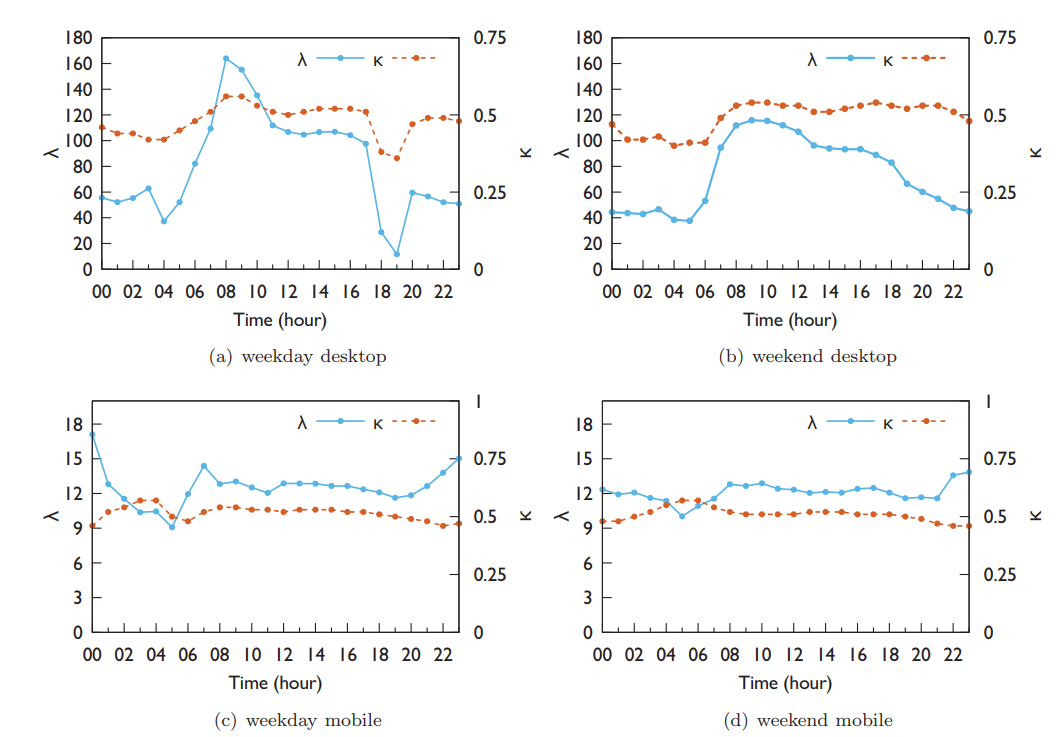
\includegraphics[height=9cm]{images/length.png}

The graphs above reveal much information about listening habits. In graph (a),
which is for desktop users during weekdays, session length peaks in the morning,
and steadily decreases until the evening. This suggests that most destop users
are playing songs on Spotify as background music during the workday.

\begin{center}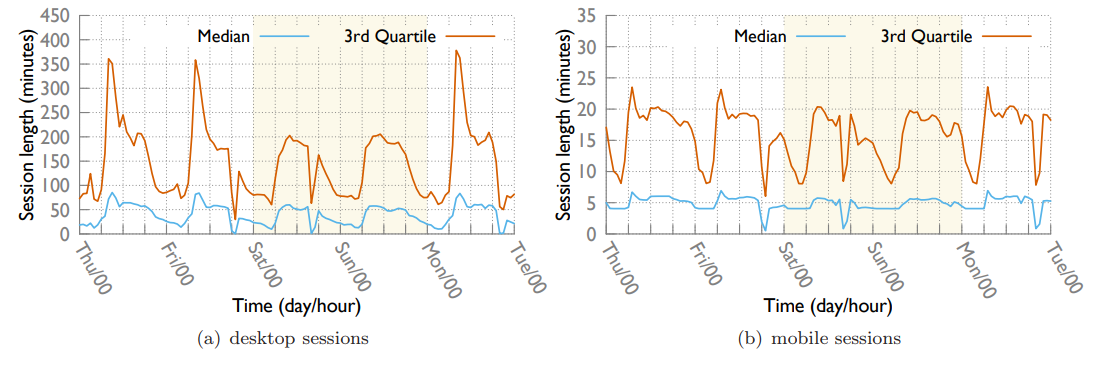
\includegraphics[height=5cm]{images/session.png}
\end{center}

The above graphs, using the same data, show that on average, mobile sessions
are shorter than their desktop companions. In addition, the morning peak is not
as pronounced, and there is more overall variation. Since these graphs suggest
a difference in listening habits between mobile and desktop, reflecting these
practices in Scottipy is an intriguing task. Since desktop sessions tend to
be longer, it may be fruitful to increase the default number of songs generated
for the platform. On mobile, it would be worthwhile to investigate tailoring
the list to shorter playlists, perhaps by involving song popularity, or other
efforts that could simultaneously lower the amount of music, but make each track
more meaningfully chosen by the data metrics Spotify gives.

\section{Conclusion}
The data that The Echo Nest and Spotify have aggregated makes finding new music
the easiest that it has ever been. Despite this, music discovery on the Spotify
platform is currently limited to just one weekly static playlist. The project
I have outlined will allow music listeners to harness the data that Spotify posesses,
in the hopes of finding unfamiliar but enjoyable music. This project aims to make
music discovery a more easy and rewarding task than currently possible.
